\subsection{Argument Identification (vs. SRL and ReVerb)}
\label{sec:ai}
%Take another corpus and parse it with dependency parser, have human label the
%correctness. We may need to artificially inject errors if there's not enough
%incorrect action instances. Now use our lexicon, ReVerb and SRL to verify
%the correctness and then compare the correlations with the human labels.
%
%If a sentence contains logically or syntactically incorrect argument, then
%the method is supposed to identify that.
%
In the argument identification task, we use our lexicon to examine
whether an argument is correct to a verb in a sentence.
In this paper, we focus on identifying the objects of a verb. To evaluate
the accuracy of argument identification, we first generate a set of
annotated \pair{verb}{obj} pairs from sentences extracted from Wikipedia
articles. Since using wrong argument in human writing is a rare case in daily life, especially
for the high quality online Encyclopedia, the
negative examples of \pair{verb}{obj} pairs are dominated by the positive
ones, which makes it difficult to observe the real differences in accuracy
among the lexicons. We thus generate artificial negative examples as follows.
First, we sample 1000 sentences that contains the verbs in
Verb-20 from Wikipedia and extract action instances from it. Then, we
randomly exchange the arguments with arguments of any other verb. For
example, we exchange ``clothing'' in ``wear clothing'' with the ``piano''
in ``play piano'' and get two negative examples ``wear piano''
and ``play clothing''.
We repeat this exchange process several times. Finally, we manually
label the correct arguments in the 1000 sentences, and we obtain a test set
containing about 50\% negative examples.

%We generate a new dataset consists of 1000 items within each containing a sentence, (target verb,obj) pair and human label.
%First we produce a new corpus consists of sentences randomly selected from Wikipedia for
%verbs in Verb-20.
%Then we randomly select 50 sentences for each target verb in which the verb's direct object exists.
%All the direct objects are collected and for each sentence,
%an alternate object is sampled from the object set.
%We switch the origin direct object and the newly sampled
%one in the sentence and assure that the alternate is still parsed as the verb's object.
%Finally, the new verb-obj pairs are manually labelled for plausible or not.


We compare our lexicon with SP, ReVerb and SRL as follows:
\begin{itemize}
\item {\bf AC \& SP}: Check if the object is an instance of the top $k$ concepts of the target verb.
\item {\bf ReVerb}: Check if the object is contained in the object list of the target verb in ReVerb.
\item {\bf SRL}: We use SRL tool ``Semafor''\cite{chen2010semafor}
to label the sentence with frame defined by FrameNet,
then we check if the object is labeled as a frame element of the target verb.
\end{itemize}

\begin{figure}[th]
\centering
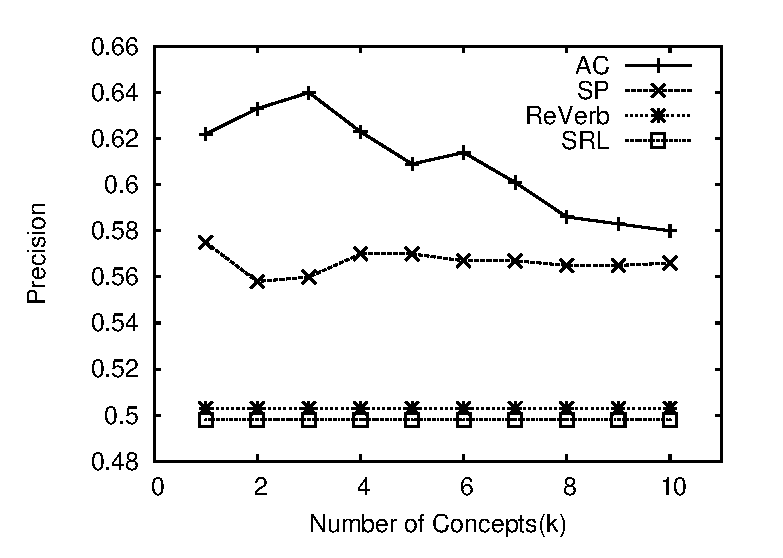
\epsfig{file=figure/argument_identify.eps,width=.65\columnwidth}
\caption{Precision of Argument Identification}
\label{fig:argumentidentify}
\end{figure}

%\KZ{Add discussion on why SRL and Reverb are bad..}
We can see from Figure \ref{fig:argumentidentify} that
the precision of AC is significantly higher than the precision of ReVerb and SRL,
and ReVerb is slightly higher than SRL.
ReVerb, due to its limited scale,  cannot recognize many argument
instances in the test data, and thus often labels true arguments
as negative. SRL, on the opposite side, tends to label everything
as positive because the SRL classifier is trained based
on features extracted from the context, which remains the same
even though we exchange the arguments. Thus SRL still labels the
argument as positive. In AC, the precision is higher with smaller $k$,
indicating high quality concepts are ranked high in our algorithm.
Precision becomes stable when $k$ reaches 7.

